\documentclass[10pt,a4paper,twocolumn]{article}
\usepackage[margin=2cm,columnsep=0.7cm]{geometry}
\usepackage{amsmath,amssymb,amsthm}
\usepackage{booktabs}
\usepackage{graphicx}
\usepackage[expansion=false]{microtype}
\usepackage{xcolor}
\usepackage{enumitem}
\usepackage[font=small,labelfont=bf]{caption}
\usepackage[colorlinks,linkcolor=blue!60!black,citecolor=blue!60!black,urlcolor=blue!60!black]{hyperref}
\hypersetup{pdftitle={Verifying Decisions Under Uncertainty: A Value-Aware Evaluation Framework for Sequential Language-Model Agents},pdfauthor={Imen Al Samarai}}
\usepackage{tcolorbox}
\setlist{nosep,leftmargin=1.2em}
\raggedbottom
\newcommand{\J}{J}
\newcommand{\ON}{\textsc{on}}
\newcommand{\OFF}{\textsc{off}}
\newcommand{\sigz}{\sigma_z}
\newcommand{\sigx}{\sigma_x}
\newtcolorbox{cotbox}{colback=gray!6,colframe=gray!40,boxrule=0.4pt,arc=1pt,left=4pt,right=4pt,top=3pt,bottom=3pt,fontupper=\small\ttfamily}

\title{\vspace{-1.2em}Verifying Decisions Under Uncertainty:\\A Value-Aware Evaluation Framework for Sequential Language-Model Agents}
\author{Imen Al Samarai\\\small Independent Researcher, Paris, France\\\small\texttt{imen.alsamarai@gmail.com}\\\small ORCID: \href{https://orcid.org/0009-0001-0060-9225}{0009-0001-0060-9225}}
\date{\small October 2026}

\begin{document}
\maketitle

\begin{abstract}
\noindent Evaluating language-model agents in sequential environments remains challenging when rewards are stochastic and decisions have consequences beyond the current step. Realised outcomes conflate decision quality with chance, while action accuracy overlooks the economic significance of errors. We introduce a value-aware evaluation framework that uses stochastic optimal control to quantify the expected value lost at each decision and attribute these losses to overall policy performance. We instantiate the framework in a financially motivated optimal-switching benchmark, where agents repeatedly decide whether to activate or deactivate a trading strategy as market signals evolve, subject to switching costs. A Bellman-optimal reference provides the expected value of each available action, enabling decision-level verification and a decomposition of expected policy regret.

We evaluate Claude Opus~4, Sonnet~4, and Haiku~4.5 across 500 episodes each. Despite more than 90\% agreement with the optimal policy, the models' policies are close to a one-step greedy rule: they are almost always right where the immediate payoff settles the decision and almost always wrong where future consequences matter, which is where their expected losses concentrate. A planning instruction raises agreement on these decisions more than tenfold, yet much of the value it recovers there is lost on decisions the immediate payoff settles, and its net gain in expected value is small and not statistically established. These findings demonstrate how value-aware verification reveals the economic consequences of agent decisions that aggregate metrics conceal, providing a principled basis for diagnosing sequential policies and evaluating policy changes.
\end{abstract}

\section{Introduction}\label{sec:intro}

Reinforcement learning with verifiable rewards has driven rapid progress on reasoning tasks whose answers can be checked. A correctness signal alone elicits long chains of thought~\cite{deepseekr1}, and procedurally generated tasks with algorithmic verifiers extend the recipe to hundreds of domains~\cite{reasoninggym,rlve}. In each case, the object the model produces can be checked after the fact.

Decisions made under uncertainty do not share this property, because their outcomes depend on events the decision-maker does not control. An agent that keeps a trading strategy active and then sees the market turn has not necessarily decided badly, and an agent that switches off and misses a rally has not necessarily decided well. Realised reward mixes the expected quality of a decision, given what was known when it was made, with the variation introduced by what happened next; averaging over episodes reduces the second component but cannot reveal which decisions produced the result. Fields that evaluate such decisions have long separated the quality of a decision from its outcome. Weather forecasts are judged by their value to the decisions they inform as well as by their accuracy~\cite{murphy1993,richardson2000}, classifiers by the cost of their errors rather than their number~\cite{elkan2001}, clinical prediction models by their net benefit~\cite{vickers2006}, and trade executions by their shortfall against the price at the moment of decision~\cite{perold1988}.

Language-model agents increasingly act in this setting, yet they are still evaluated mainly by outcomes. Agent and game suites score completed episodes~\cite{agentbench,mint,smartplay,balrog}, financial benchmarks score realised profit~\cite{kellybench,livetradebench,stockbench}, and bandit studies measure cumulative regret~\cite{krishnamurthy2024,nie2024evolve,park2024regret}. Where an optimal policy is known, it serves to normalise episode returns~\cite{agentick,llmsdm2026}, to compare trajectories in deterministic environments~\cite{costbench}, or to score single-period orders~\cite{aimbench,llmnewsvendor}. Models have also been evaluated on classical planning~\cite{planbench} and one-shot decisions under uncertainty~\cite{dellma}, and step-by-step reasoning has been found to produce greedy policies over long horizons~\cite{whyreasoningfails}. Action values conditioned on the state are standard in dynamic programming, but to our knowledge they have not been used to evaluate each decision a language-model agent makes in a stochastic environment, to attribute its regret by decision class, or to evaluate changes to its policy.

\paragraph{Approach.} We evaluate decisions against a mathematical reference rather than against outcomes. For problems in stochastic optimal control, finite-horizon dynamic programming gives the optimal action at every state and the expected value of each alternative under the true data-generating process. Each decision can therefore be compared with that expectation, its cost measured in value rather than counted as an error, and the costs summed into the agent's expected shortfall as a policy. The agent receives what a deployed agent would receive, namely the payoff rules and the history of the signal, and the framework measures the expected value of the decisions it makes with that information. We instantiate the framework on optimal switching with a fixed cost on a mean-reverting signal, a canonical problem in quantitative finance~\cite{brekke1994,zervos2003,hamadene2007,lyvath2007,leung2015}.

\paragraph{Contributions.} The paper makes three contributions. First, it defines the framework: Bellman action values as a per-decision reference, decision classes defined by whether future value changes the optimal action, and a decomposition of expected policy regret into those classes (\S\ref{sec:method}). Second, it provides a validated benchmark instance, with numerical checks and a map of where consequential decisions arise (\S\ref{sec:bench}--\ref{sec:validation}). Third, it demonstrates the framework's two uses on three frontier models: diagnosing where a policy loses expected value, and evaluating whether a change to the agent improves it (\S\ref{sec:eval}). The models' greedy tendency is anticipated by prior work~\cite{whyreasoningfails}; the framework measures where that tendency costs them, by how much, and how an intervention changes the account.

\section{The Optimal-Switching Benchmark}\label{sec:bench}

\paragraph{Design principle.} The framework requires three properties of an environment: stochastic outcomes, an optimal policy computable to numerical precision, and online interaction with the agent. Several classical control problems have these properties, including optimal stopping, inventory control with persistent demand and execution with price impact. This paper implements one of them, optimal switching, which has a direct financial interpretation.

\paragraph{Financial motivation.} Consider a quantitative strategy that can be active or inactive. Its expected payoff depends on a signal, such as a spread, a valuation gap or an indicator of temporary mispricing, which evolves stochastically and reverts toward a long-run level. Because activating or deactivating the strategy has a cost, the relevant comparison is not between today's payoff and the cost, but between acting now and holding through the signal's expected path on the one hand, and waiting on the other. The decision therefore depends on future opportunities as well as on the current signal. The Ornstein--Uhlenbeck (OU) process is a standard reduced-form model of such a signal~\cite{elliott2005,bertram2010,leung2015}.

\paragraph{Environment.} At each step $t=0,\dots,T{-}1$ the agent observes $z_t$ and chooses $s_t\in\{0,1\}$ (\OFF/\ON). Being \ON{} earns the realised payoff $x_t$, each switch costs $\lambda$, and the initial position $s_{-1}$ is drawn uniformly and shown to the agent. Utility is
\begin{equation}
\J(\mathbf{s})=\sum_{t=0}^{T-1}\Big[s_t\,x_t-\lambda\,\mathbf{1}\{s_t\neq s_{t-1}\}\Big],
\label{eq:J}
\end{equation}
and the signal follows
\begin{equation}
z_{t+1}=(1-\kappa)\,z_t+\sigz\,\varepsilon_t,\qquad \varepsilon_t\sim\mathcal N(0,1),
\label{eq:ou}
\end{equation}
with $z_0\sim\mathcal N(0,\sigz^2/(2\kappa))$, the continuous-time stationary variance used by the released generator. The exact discrete value, $\sigz^2/(2\kappa-\kappa^2)$, is at most 14.3\% larger over the evaluation range; the difference changes where episodes start, not the optimal policy or its action values. The payoff is $x_t=\alpha z_t+\sigx\eta_t$ with $\eta_t\sim\mathcal N(0,1)$, so the signal determines the conditional expected payoff $\alpha z_t$ and $\sigx\eta_t$ is the component that no decision could anticipate. An instance is defined by $(\kappa,\sigz,\sigx,\alpha,\lambda,T)$ and the initial position $s_{-1}$, and the ratio $r=\lambda/\alpha$ is the threshold that a one-step comparison of payoff against cost applies to $z_t$.

\paragraph{Agent protocol.} The agent plays $T$ turns in one conversation. A system prompt states $(\alpha,\lambda,T,s_{-1})$, each turn presents $t$, $z_t$ and the current position, and the agent replies with $s_t$ (Appendix~\ref{app:prompts}); it observes the signal and the expected-payoff rule, not the realised payoffs $x_t$. Earlier turns remain in context, so the agent sees the full signal history and its own past decisions, but not future values, the dynamics~\eqref{eq:ou}, or the fact that the signal mean-reverts. Recognising from the history that the signal persists is therefore part of the task, as it is for a deployed agent, which is rarely told the dynamics of the signals it acts on; the information set is the same for every policy compared in \S\ref{sec:eval}. The reference, in contrast, knows the dynamics and their parameters. It is therefore an omniscient benchmark rather than the best policy attainable from the agent's information, and \S\ref{sec:stakes} measures the difference between the two.

\paragraph{Problem instances.} Parameters are drawn independently for each episode, and each one shapes the decision differently. Persistence (small $\kappa$) makes a favourable signal informative further ahead, volatility raises the chance that it reverses before a cost is recovered, $r$ sets how strong a signal must be before a one-step rule acts, and $T$ bounds the time available to amortise a cost. The \emph{evaluation regime} draws $\kappa\sim U[0.1,0.25]$, $r\sim U[0.3,0.5]$, $\alpha\sim U[0.1,0.5]$, $\sigz,\sigx\sim U[0.1,0.3]$ and $T\sim U\{5,\dots,20\}$; the payoff noise $\sigx$ affects realised utility but neither the optimal action nor what the agent observes. In this regime the immediate payoff settles most decisions, while about 9\% of the decisions the evaluated models reach depend on future value, which provides enough decisions of each kind for statistical comparison. Figure~\ref{fig:episode} shows one episode, and \S\ref{sec:validation} maps the wider parameter space.

\begin{figure}[t]
\centering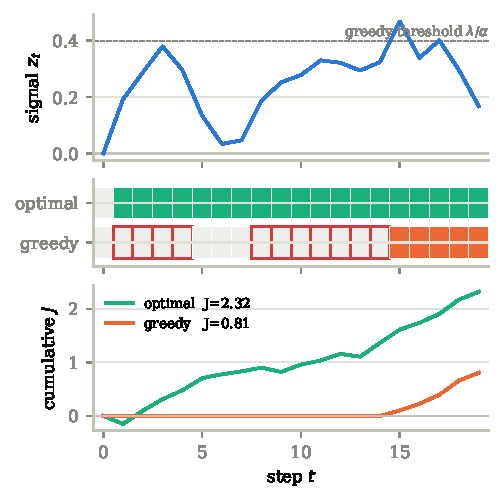
\includegraphics[width=\linewidth]{fig1_episode.pdf}
\caption{Example evaluation-regime episode ($\kappa{=}0.15$, $r{=}0.4$, $\alpha{=}0.37$, $T{=}20$, $\sigz{=}\sigx{=}0.1$, $z_0{=}0$, $s_{-1}{=}\OFF$). Top: signal and greedy threshold. Middle: optimal vs.\ greedy actions (filled\,=\,\ON); red borders mark continuation-sensitive decisions in the states the greedy agent reaches. Bottom: cumulative realised utility. Optimal switches on at $t{=}1$ when $z_t$ is half the greedy threshold, holds through the dip, and amortises the cost over 19 steps ($J{=}2.32$); greedy waits until $z_t>r$ at $t{=}15$ ($J{=}0.81$).}
\label{fig:episode}
\end{figure}

\section{Decision-Level Verification and Regret}\label{sec:method}

\paragraph{Bellman-optimal reference.} The reference is the solution of the finite-horizon Bellman equation. With $V_T\equiv0$, actions $a\in\{0,1\}$ and the expectation taken over~\eqref{eq:ou},
\begin{equation}
V_t(z,s)=\max_{a}\Big[a\alpha z-\lambda\mathbf 1\{a\neq s\}+\mathbb E\big[V_{t+1}(z',a)\mid z\big]\Big].
\label{eq:bellman}
\end{equation}
Backward induction with 20-node Gauss--Hermite quadrature on a 200-point grid yields the action values $Q_t(z,s,a)$ of both actions at every state and the optimal policy $\pi^*=\arg\max_a Q$ (Appendix~\ref{app:verify-solver}). The payoff noise has zero mean and does not enter~\eqref{eq:bellman}, so it affects realised utility but not the optimal action. The language model is never asked to solve the equation; the solution serves only as the evaluator's instrument.

\paragraph{Evaluation metrics.} Two decision-level measurements complement the outcome measure. \emph{Realised utility}, the mean of~\eqref{eq:J}, is what deployment observes, but it mixes decision quality with chance. \emph{Optimal-action agreement} is the fraction of decisions that match $\pi^*$ in the state actually reached. \emph{Expected decision-level regret},
\[
\Delta_t=Q_t(z_t,s_{t-1},a^*_t)-Q_t(z_t,s_{t-1},a_t),
\]
is the expected value given up by choosing $a_t$ instead of the reference action $a^*_t$, assuming optimal play thereafter (Appendix~\ref{app:verify-solver} specifies how $a^*_t$ and $Q_t$ are computed). Whereas agreement counts errors, regret weighs them: two wrong actions may be a near-tie and a large loss, and only regret distinguishes them.

\paragraph{Decision classes.}\label{sec:classes} The decision classes follow from removing the continuation term in~\eqref{eq:bellman}. The resulting one-step greedy rule switches \ON{} if $\alpha z_t>\lambda$, switches \OFF{} if $\alpha z_t<-\lambda$, and otherwise keeps the current position. Where this rule agrees with $\pi^*$, the decision is \emph{greedy-consistent}, because the immediate payoff settles it. Where it disagrees, the decision is \emph{continuation-sensitive}, because future value changes the optimal action, and a one-step rule gets it wrong by construction. The class is a property of the state, evaluated at the state the agent reached, and it describes where a policy's errors fall rather than how the agent reasoned. For this reason agreement and regret are always reported together for each class.

\paragraph{From decisions to policy regret.}\label{sec:regret} The finite-horizon performance-difference identity connects decision-level regret to policy performance. For any policy $\pi$,
\begin{equation}
V^*_0(z_0,s_{-1})-V^{\pi}_0(z_0,s_{-1})=\mathbb E_{\pi}\Big[\textstyle\sum_{t}\Delta_t\Big],
\label{eq:pdl}
\end{equation}
where the expectation is over the states that $\pi$ itself visits. Summing $\Delta_t$ along a logged trajectory therefore gives an unbiased estimate of the policy's expected shortfall from the optimum, and the sum splits exactly into a greedy-consistent part $R_{\rm GC}$ and a continuation-sensitive part $R_{\rm CS}$. Expected regret differs from the realised gap $\J_{\rm opt}-\J_\pi$, which also contains payoff noise, the particular signal paths drawn and sampling error; the two agree in expectation. Because~\eqref{eq:pdl} integrates over each policy's own states, a difference in regret between two policies is a difference in expected performance; \S\ref{sec:casestudy} complements it with a comparison at identical states.

\paragraph{Horizon-response diagnostic.} Under $\pi^*$, a switching cost is worth paying only if enough time remains to recover it, so at a given signal strength the optimum switches in more states the longer the remaining horizon. The greedy rule, by contrast, ignores the horizon. A regression of an agent's switches on the remaining horizon, controlling for signal strength, position and parameters, therefore tests whether its policy has the optimal shape. Since simple horizon-aware rules also produce a positive response (Appendix~\ref{app:verify-heur}), the test characterises the form of a policy rather than the computation behind it.

\section{Validation of the Reference}\label{sec:validation}

Before evaluating any model, we establish that the reference is numerically reliable and that the decisions it identifies as consequential carry real value.

\paragraph{Numerical stability.}\label{sec:numerics} We re-solved every evaluation episode with finer discretisations and compared actions, classes and action-value gaps at the 6{,}197 states visited by Claude Opus~4. Grids of 400 or 800 points change the optimal action at one state at most (0.02\%) and the gap by at most 0.8\% of $\lambda$. Doubling the quadrature to 40 nodes changes five actions (0.08\%) and the gap by at most 2.1\% of $\lambda$, combining both refinements changes the same five, and widening the grid changes none. Every affected state lies within $0.03\lambda$ of a tie, so the classification is stable and the regret figures reported below are unaffected at the second decimal. The same holds outside the evaluation regime, where large switching costs can place the greedy threshold $r$ beyond the released grid and constant extrapolation could distort continuation values. Re-solving with a grid of half-width $\max(12$ exact standard deviations$,\,3r)$, 1{,}600 points, and linear instead of constant extrapolation beyond its edges changes 0.2\% of actions in the high-cost regime introduced below (400 simulated episodes), each within $0.012\lambda$ of a tie, and no state visited in these episodes lies beyond the original grid.

\paragraph{Difficulty characterisation.}
\begin{figure*}[t]
\centering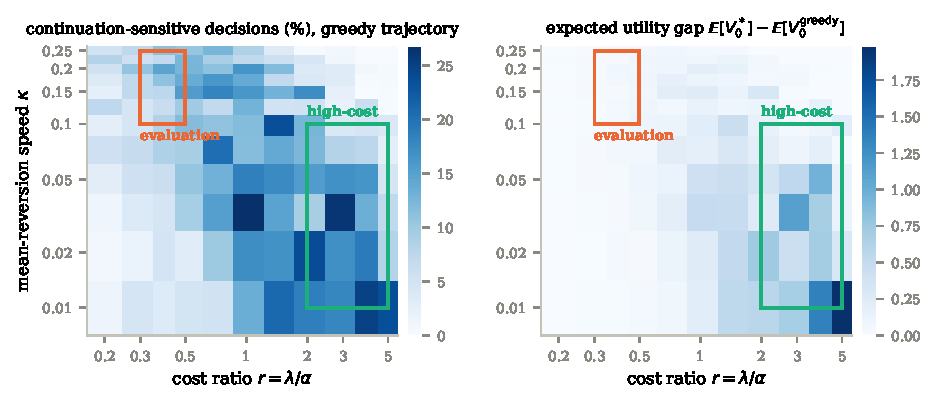
\includegraphics[width=\textwidth]{fig2_surface.pdf}
\caption{Difficulty surface over $(\kappa, r)$ with $\alpha,\sigz,\sigx,T,s_{-1}$ drawn from the evaluation-regime distributions (30 episodes per cell; cells are centred on the sampled values, logarithmic axes). \textbf{Left:} fraction of continuation-sensitive decisions in the states a greedy agent reaches. \textbf{Right:} expected utility gap between the optimum and the greedy rule, i.e.\ the greedy rule's expected regret along its own trajectory. Boxes mark the evaluation regime ($\kappa\in[0.1,0.25]$, $r\in[0.3,0.5]$) and the high-cost regime ($\kappa\in[0.01,0.10]$, $r\in[2,5]$) at their exact boundaries. Continuation-sensitive decisions concentrate on a ridge where $r$ is comparable to the signal scale and reversion is slow; the expected gap grows toward slow reversion and large $r$, where the decisions that differ are worth a great deal.}
\label{fig:surface}
\end{figure*}
The parameter space determines how often future value matters and how much it is worth. Figure~\ref{fig:surface} maps $(\kappa,r)$ by the fraction of continuation-sensitive decisions along greedy trajectories and by the expected utility gap between the optimum and the greedy rule. Continuation-sensitive decisions concentrate on a ridge where $r$ is comparable to the signal's stationary scale and persistence is high. Below the ridge the greedy rule switches readily and agrees with the optimum, above it neither policy switches, and along it, increasingly as $\kappa\to0$, the greedy rule switches too rarely. The value of these decisions therefore depends strongly on the regime. Over 2{,}000 simulated episodes each, the greedy rule forgoes 17\% of the optimal expected utility in the evaluation regime (expected regret $0.058\pm0.002$ against $\mathbb E[V^*_0]=0.352$; on the 500 episodes of \S\ref{sec:eval}, 0.052 against 0.342) and practically all of it in a high-cost regime with $\kappa\in[0.01,0.10]$, $r\in[2,5]$ and the other parameters as in the evaluation regime ($0.45\pm0.03$ against 0.45), although continuation-sensitive decisions are only slightly more frequent there (13\% against 10\% of the states along greedy trajectories). The generator thus controls both the frequency and the value of consequential decisions. We use expected rather than realised utility for this comparison because realised utility in the high-cost regime is dominated by noise from slowly reverting signals.

\paragraph{Value at stake.}\label{sec:stakes}
\begin{figure*}[t]
\centering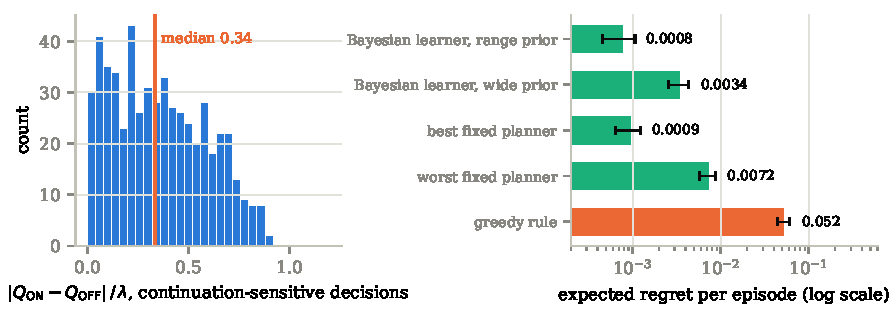
\includegraphics[width=\textwidth]{fig3_kappa.pdf}
\caption{Value at stake and the cost of not knowing the dynamics' parameters. \textbf{Left:} $|Q_{\ON}-Q_{\OFF}|$ normalised by the switching cost at the 551 continuation-sensitive decisions Claude Opus~4 encountered; the median is 0.34 and only 7\% of these decisions are within 0.05 of a tie. \textbf{Right:} expected regret per episode on the 500 evaluation episodes, each policy along its own trajectory, with 95\% intervals. The Bayesian learners have the agent's information and learn $(\kappa,\sigz)$ online, from a prior on the evaluation ranges or from a wide prior spanning a near-random walk to white noise; the fixed planners act on wrong but fixed values on a $3{\times}3$ grid over the evaluation ranges (Appendix~\ref{app:verify-kappa}). Each costs a small fraction of the greedy rule's regret and of the models' regret of 0.043--0.047 (Table~\ref{tab:results}).}
\label{fig:kappa}
\end{figure*}
Continuation-sensitive decisions are consequential rather than near-ties. At the 551 such states Opus~4 visited (including the 55 whose responses are not scored, \S\ref{sec:eval}), the normalised gap $|Q_{\ON}-Q_{\OFF}|/\lambda$ has a median of 0.34 (IQR 0.16--0.55), with 7\% within 0.05 of a tie and 16\% within 0.10 (Figure~\ref{fig:kappa}, left); Sonnet and Haiku give similar figures (medians 0.34 and 0.33).

The reference knows $\kappa$ and $\sigz$, whereas the agent does not, so the next question is how much of the measured regret this information gap could explain. A single episode is too short to estimate $\kappa$: from 8 observations the least-squares estimate of $\kappa$ has a standard deviation of about 0.3, twice the width of the evaluation range (Appendix~\ref{app:verify-kappa}). We therefore evaluate two kinds of planner without parameter knowledge on the same 500 episodes (Figure~\ref{fig:kappa}, right). Planners that act on fixed wrong values of $(\kappa,\sigz)$ disagree with the reference on up to 32\% of continuation-sensitive decisions, but these disagreements are cheap: their expected regret is 0.0009--0.0072 per episode. A Bayesian learner that receives exactly the agent's information, starts from the evaluation-regime ranges and updates its posterior over $(\kappa,\sigz)$ at every step loses $0.0008\pm0.0002$ and agrees with the reference on 95\% of continuation-sensitive decisions (measured, for all planners, on the states Opus visited). Because the episodes are drawn from those same ranges, the Bayes-optimal policy for the agent's information does at least as well as this learner in expectation, so the omniscient reference and the best attainable policy differ by no more than about 0.001 per episode, given that the signal is a persistent first-order autoregression; this is about 2\% of the models' regret of 0.043--0.047 (\S\ref{sec:eval}). The result does not rest on knowing the ranges. A learner whose prior spans every speed from a near-random walk ($\kappa{=}0.01$) to white noise ($\kappa{=}1$), with $\sigz$ from 0.03 to 1, loses $0.0034\pm0.0005$, although at the end of an episode its posterior places only a quarter of its mass on the evaluation range of $\kappa$; its low regret reflects how little the decisions depend on $\kappa$, not that it learns $\kappa$. Both learners know that the signal follows such an autoregression, and the wide prior, being logarithmic, still favours persistent signals, whereas the agent must recognise persistence from the history. This distinction matters because the greedy rule is optimal for a signal without persistence; \S\ref{sec:horizon} shows that it does not account for the models' behaviour.

\section{Evaluation of Frontier Language Models}\label{sec:eval}

We apply the framework to three frontier models for its two uses: diagnosing where a policy loses expected value, and evaluating a change to the policy. The models serve as a case study: the complete logs are released, so every result can be reproduced from the data, and the environment evaluates any other model without change to the method.

\paragraph{Protocol.} Claude Opus~4, Sonnet~4 and Haiku~4.5 were each evaluated on the same 500 episodes (6{,}197 decisions per model) under the protocol of \S\ref{sec:bench}, with the API's default sampling temperature (1.0), a maximum of 300 output tokens, no extended thinking and no tools. The decision is read as the last expression of the form $s_t=0$ or $s_t=1$ in the response (Appendix~\ref{app:prompts}). Responses that do not state a final decision within this limit are treated as invalid and excluded from scoring; they make up 3.0\%, 4.2\% and 6.3\% of the responses of Opus, Sonnet and Haiku (Appendix~\ref{app:verify-complete}). Each scored decision is evaluated at the state the model actually reached, and expected regret per episode is the sum of $\Delta_t$ over its scored decisions, that is, the expected value lost by the decisions the model stated. Since $\Delta_t\ge0$, this sum is a lower bound on the shortfall in~\eqref{eq:pdl} along the trajectories actually followed; the remaining terms belong to the excluded responses, whose parsed values come from unfinished text rather than stated decisions and are therefore not scored. Assigning each excluded decision the mean regret of the scored decisions in its class raises the default models' regret by 11--14\%. The greedy rule and the optimum are run on the same episodes.

\subsection{Diagnosis: where the models lose value}\label{sec:diagnosis}
\begin{table*}[t]
\centering\scriptsize\setlength{\tabcolsep}{3.5pt}
\resizebox{\textwidth}{!}{\begin{tabular}{@{}lcccccccc@{}}
\toprule
 & & \multicolumn{2}{c}{Optimal-action agreement} & \multicolumn{3}{c}{Expected regret per episode} & \\
\cmidrule(lr){3-4}\cmidrule(lr){5-7}
Policy & Scored decisions & greedy-consistent & continuation-sensitive & total [95\% CI] & GC & CS & Greedy action, same states \\
\midrule
Opus 4    & 6{,}012 (97.0\%) & 99.9\% (5509/5516) & 4.8\% (24/496) & 0.043 [0.036, 0.051] & 0.000 & 0.043 & 0.045 \\
Haiku 4.5 & 5{,}809 (93.7\%) & 99.9\% (5325/5328) & 0.8\% (4/481) & 0.043 [0.036, 0.050] & 0.001 & 0.042 & 0.043 \\
Sonnet 4  & 5{,}935 (95.8\%) & 99.9\% (5434/5437) & 0.2\% (1/498) & 0.047 [0.039, 0.055] & 0.001 & 0.046 & 0.046 \\
\midrule
Greedy rule & 6{,}197 & 100\% & 0\% & 0.052 [0.044, 0.060] & 0 & 0.052 & -- \\
Bellman optimum & 6{,}197 & 100\% & 100\% & 0 & 0 & 0 & -- \\
\bottomrule
\end{tabular}}
\caption{The 500 evaluation episodes, same seeds. Agreement is measured in the state each policy reached. Expected regret is summed over each policy's scored decisions along its own trajectory, with episode-level bootstrap CIs, and split into greedy-consistent (GC) and continuation-sensitive (CS) decisions; components may not sum to the total because of rounding. The last column gives the regret the greedy action would incur at the models' own scored states. The optimal expected utility is $\mathbb E[V^*_0]=0.342$. The differences between the three models are within sampling error, and we do not rank them.}
\label{tab:results}
\end{table*}

The decomposition by decision class locates the models' losses (Table~\ref{tab:results}). Agreement alone suggests near-optimal play: the models choose the optimal action in 92\% of scored decisions. Expected regret shows that they lose 0.043--0.047 per episode, 12--14\% of the optimal expected utility, and that the loss has a single source. On greedy-consistent decisions the three models agree with the optimum 99.9\% of the time, and this class contributes at most 0.001 per episode. On continuation-sensitive decisions they agree 0.2--4.8\% of the time, and this class accounts for more than 97\% of their regret. At the same states, the greedy action would lose 0.043--0.046 per episode, within 0.002 of the models' own regret. The models' policies are therefore, to a close approximation, the one-step greedy rule: reliable where the immediate payoff decides, and almost never forward-looking where the future changes the optimal action.

This diagnosis is not available from aggregate measures. An agreement rate of 92\% coincides with the share of decisions that the immediate payoff settles, and an agent that never looks ahead attains it. Expected regret weights each error by its cost, and the decomposition shows that the value at stake lies in the 8\% of decisions on which the models fail. Section~\ref{sec:stakes} established that these decisions carry a median of 0.34 switching costs each, so the failure is consequential rather than a matter of near-ties.

\subsection{Horizon response}\label{sec:horizon}
\begin{figure*}[t]
\centering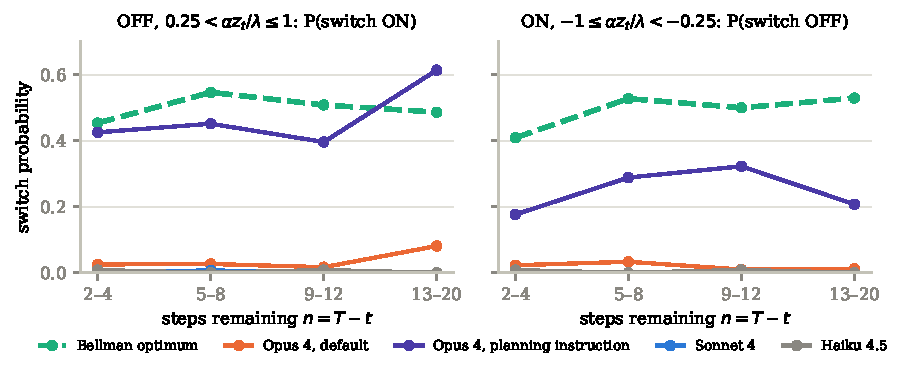
\includegraphics[width=\textwidth]{fig4_horizon.pdf}
\caption{Switch probability as a function of the steps remaining $n=T-t$, in the band of signal strengths where the greedy rule never switches and the reference often does (scored decisions; $N{=}500$ episodes per series). The final step, where the reference coincides with the greedy rule, is excluded. The reference's switch probability rises with the horizon because a switching cost needs time to be amortised; the default models rarely switch in this band at any horizon. The instructed model switches more often at every horizon, and more readily \ON{} from \OFF{} than \OFF{} from \ON{}, although the problem is symmetric (Appendix~\ref{app:verify-heur}); this is consistent with the prompt, which describes \OFF{} as earning nothing, and with the instruction's reference to ``future gains''.}
\label{fig:horizon}
\end{figure*}
The horizon diagnostic confirms that the models do not amortise switching costs. It uses the band of signal strengths where the greedy rule never switches and the optimum often does, $0.25<\alpha z_t/\lambda\le1$ when \OFF{} and $-1\le\alpha z_t/\lambda<-0.25$ when \ON{}, and excludes the final step, where the optimum coincides with the greedy rule. On these states we fit a logit of the switch indicator on the number of steps remaining, $n=T-t\in\{2,\dots,T\}$, controlling for signal strength, $\kappa$, $\lambda/\alpha$, $T$, $\sigz$ and position, with standard errors clustered by episode (Appendix~\ref{app:verify-horizon}). The optimum switches in 40--43\% of band states with 2--4 steps left and in 50--56\% with more, and its coefficient on $n$ is $+0.25$ to $+0.28$ ($\pm0.05$). The default models switch in 0.1--2.9\% of band states, with no comparable rise as the horizon lengthens (Figure~\ref{fig:horizon}); Sonnet and Haiku switch in 1 and 4 of about 1{,}000 such states, so the conclusion rests on these proportions, and Opus's coefficient does not differ from zero at the 5\% level. This greedy policy does not reflect uncertainty about whether the signal persists. Agreement on continuation-sensitive decisions does not rise as the history lengthens: it remains between 0\% and 5.1\% from step 5 onwards, including late in episodes, where a simple statistical test would already reject pure noise in most cases, and decisions from step 5 onwards account for 52--58\% of the default models' continuation-sensitive regret (Table~\ref{tab:bystep}; Appendix~\ref{app:verify-kappa}). Their policies thus apply a fixed one-step threshold regardless of the time left to recover a cost.

\subsection{Evaluating a change: a planning instruction}\label{sec:casestudy}
\begin{table*}[t]
\centering\scriptsize\setlength{\tabcolsep}{6pt}
{\begin{tabular}{@{}lccc@{}}
\toprule
 & Default & Instruction & Difference [95\% CI] \\
\midrule
\multicolumn{4}{@{}l}{\emph{Agreement with the optimal action}} \\
\quad continuation-sensitive (174) & 4.6\% & 52.9\% & \\
\quad greedy-consistent (3{,}922) & 99.9\% & 98.2\% & \\
\multicolumn{4}{@{}l}{\emph{Expected loss per decision}} \\
\quad continuation-sensitive & 0.0437 & 0.0190 & $-0.0247$ [$-0.0308$, $-0.0191$] \\
\quad greedy-consistent & 0.00005 & 0.00076 & $+0.00072$ [$+0.00046$, $+0.00100$] \\
\quad all (4{,}096) & 0.00190 & 0.00154 & $-0.00036$ [$-0.00075$, $+0.00002$] \\
\bottomrule
\end{tabular}}
\caption{Opus~4 with and without the planning instruction at the 4{,}096 identical states where both responses are scored (66\% of decision pairs). Episode-level bootstrap CIs.}
\label{tab:casestudy}
\end{table*}
The diagnosis suggests an intervention, and the framework evaluates it. We appended one sentence to Opus's system prompt, \emph{``Consider the signal trend, remaining horizon, and whether paying the switching cost now will be recovered by future gains,''} and re-ran the same 500 episodes. Because the signal paths are exogenous and the seeds are shared, the two runs face identical states whenever their previous positions coincide. We compare them at the 4{,}096 identical states where both responses are scored, which evaluates both policies on the same decisions; the instruction lengthens responses, and 20\% of them are invalid under the rule of \S\ref{sec:eval}, including half of those on continuation-sensitive decisions (Appendix~\ref{app:verify-complete}).

The instruction changes the policy substantially (Table~\ref{tab:casestudy}). Agreement on continuation-sensitive decisions rises from 4.6\% to 52.9\%, more than tenfold, while agreement on greedy-consistent decisions falls from 99.9\% to 98.2\%. The framework values both effects. Where the future matters, the expected loss per decision falls by 0.025; where the immediate payoff settles the decision, it rises by 0.0007. Both changes are clearly significant. Nearly all of the new errors are switches the optimum does not make, on signals too weak to recover the cost (83 of 87 among all scored decisions), and three quarters of their cost comes from leaving \ON{}, mostly after a fall in the signal. Because greedy-consistent decisions are 22 times as frequent, the second effect offsets about two thirds of the first, and the net change in expected loss, $-0.00036$ per decision ($p{=}0.06$), is not statistically distinguishable from zero. Invalid responses are more frequent on continuation-sensitive decisions under the instruction, so these decisions make up 4.2\% of the matched states against 8.3\% of the scored decisions in the default run, and the surviving ones need not be typical of the class. Weighting the per-class changes by the full-sample mix gives a larger net change, about $-0.0014$ per decision, with the losses on greedy-consistent decisions offsetting about a third of the gain. The excluded continuation-sensitive decisions resemble the scored ones, with a median value at stake of 0.36 switching costs against 0.31 and the same mean step. Under either weighting, expected loss falls far less than the tenfold rise in targeted agreement suggests. Both runs share the 300-token limit, so the instruction is evaluated under it; since the instruction lengthens responses, a larger limit might recover more of the targeted decisions.

The instruction raises the propensity to switch more than it conditions switching on the horizon. In the band of \S\ref{sec:horizon}, the instructed policy switches in 28--42\% of its scored states, against 34--53\% for the optimum, with a horizon coefficient of $+0.045\pm0.025$ ($p{=}0.07$). At the 384 matched band states, the change in horizon response relative to the default is $-0.014\pm0.083$, against a main effect of $+3.6$ on the log-odds of switching. Its agreement on continuation-sensitive decisions is already 57\% at the first two steps, before the history can reveal persistence, so the instruction, which mentions the signal trend, supplies the expectation that the signal persists as well as the prompt to look ahead.

The case study illustrates the framework's second use. The metric the instruction targets improves more than tenfold, and an evaluation based on agreement would adopt it. The value accounting shows that the gain is real where the future matters but is partly spent on new errors where it does not, leaving a net improvement too small to establish with 500 episodes. Deciding whether to adopt such a change requires exactly this accounting: the value recovered on the targeted decisions, the value lost elsewhere, and their difference.

\section{Discussion and Limitations}\label{sec:limits}

\paragraph{Implications for agent evaluation.} Decision-value verification complements outcome evaluation by supplying the expected value of each decision. Realised reward remains what deployment produces, and~\eqref{eq:pdl} ties the two levels together: the expected shortfall that outcomes estimate in aggregate is the sum of the action-value gaps of individual decisions. This connection allows an evaluator to attribute a policy's shortfall to classes of decisions and to determine which decisions a modification changed and in which direction. Outcome scores, agreement rates and the agent's stated reasoning, which need not reflect the computation behind an action~\cite{turpin2023}, do not provide this attribution.

\paragraph{Application to financial agents.} The benchmark corresponds to decisions that a financial agent makes when it activates a strategy, holds a position through adverse readings, or exits. For such an agent, the action-value gap serves as an audit quantity: it measures what each decision cost in expectation, under a stated model, relative to the best alternative, and it can be accumulated over a decision log and attributed to decision classes. Model-based decision auditing of this kind complements profit monitoring, which measures outcomes, and risk management, which bounds exposure, by evaluating individual decisions. Because the benchmark's signal is a stylised model, its conclusions are conditional on that model and do not measure any agent's performance in real markets.

\paragraph{Application to verifiable reinforcement learning.} The same action-value gaps are a candidate training signal. A realised-outcome reward credits a decision with what happened afterwards, which in a stochastic environment is noisy and partly outside the agent's control, whereas the action-value gap credits it with its expected consequence and is zero exactly when the decision is optimal. The environment exposes the quantities needed to construct such value-aware training signals for Gym-style reinforcement-learning pipelines; whether they improve post-training remains to be tested.

\paragraph{Scope.} The results are bounded by the benchmark and the protocol. One task family is implemented, and although the construction applies to other stochastic control problems, its diagnostic value there has not been tested. Exact verification also requires a reference that can be computed to numerical precision, which backward induction on a grid provides only for low-dimensional states; the cost grows exponentially with the state dimension, so richer environments would need problems with analytical structure or approximate references with error bounds. The model results hold for the evaluated configurations: three models from one family, one sampled response per state at the default temperature, a 300-token output limit, no tools, no extended thinking and the information set of \S\ref{sec:bench}. Other model families, extended thinking, a larger output limit, a symmetrically worded instruction and disclosure of the dynamics are changes that the framework evaluates in the same way as the planning instruction. Responses without a stated decision are excluded from scoring; because they occur more often under the planning instruction, the instruction is evaluated at identical states where both responses are scored. The reference is optimal under the stated OU dynamics; within this task it is within about 0.001 per episode of the best policy available from the agent's information (\S\ref{sec:stakes}), but it says nothing about optimality under an unknown real-world process. Finally, the framework characterises realised policies and the expected value of their decisions; it does not identify the models' internal reasoning.

\section{Conclusion}
Where an answer can be checked, verification compares the output with the truth; where a decision is taken before the future is known, its realised outcome is an unreliable guide to its quality, and evaluation can instead compare the decision with the expected value of its alternatives. A stochastic-control reference supplies that expectation. On a financially motivated switching task, Bellman action values verify each decision at the state the agent reached, measure its expected cost, and sum these costs into the agent's expected policy regret, which can be attributed to decisions the immediate payoff settles and to decisions on which the future changes the answer.

Applied to three frontier models, the framework serves two purposes. As a diagnostic, it shows that their policies are close to the one-step greedy rule, with nearly all of their expected loss on the 8\% of decisions where the future changes the optimal action. As an evaluation of change, it shows that a planning instruction which raises agreement on those decisions more than tenfold recovers value there but loses between a third and two thirds of it, depending on the weighting, on decisions the immediate payoff settles, leaving a net improvement that 500 episodes do not establish. Extending the benchmark to further stochastic tasks and using action-value gaps as a decision-level training signal are natural next steps.

\section*{Reproducibility}
The environment, Bellman solver, evaluation scripts, per-step logs for all $N{=}500$ runs, and the code for every analysis of the benchmark and for every figure are released at \url{https://github.com/ImenAlSamarai/decision-level-evaluation} (release \texttt{v1.0.0}). Every analysis based on the reference (\S\ref{sec:validation}--\ref{sec:eval}) runs from the released logs and solver without model calls.

\appendix
\section{Qualitative Response Examples}\label{app:cot}
The following Claude Opus~4 responses illustrate an explicitly forward-looking decision and the more common one-step pattern. Because a stated argument need not cause the action~\cite{turpin2023}, they illustrate the policies rather than explain them.

\paragraph{Example 1: an explicitly forward-looking response (seed 31, $t{=}2$).} Signal $z_2{=}0.2313$, position \OFF; parameters $\kappa{=}0.17$, $\alpha{=}0.3691$, $\lambda{=}0.1607$, $T{=}16$. Bellman-optimal: \ON; greedy: \OFF{} ($\alpha z_t{=}0.0854<\lambda$). The model overrides the greedy rule:
\begin{cotbox}
This is a stronger positive signal. I've now seen three consecutive positive signals: 0.1295, 0.1300, and 0.2313. The current signal alone generates expected profit of 0.0854, which is about 53\% of the switching cost.

With 14 steps remaining and a pattern of positive signals emerging, it may be worth switching ON now. If signals remain positive for even 2--3 more periods, I'll more than recover the switching cost.

s\_t = 1
\end{cotbox}
The response states the horizon (``14 steps remaining'', counting the current one) and an amortisation argument (``2--3 more periods'') as the basis for overriding the one-step arithmetic. 

\paragraph{Example 2: the one-step pattern (seed 223, $t{=}4$).} Signal $z_4{=}0.1539$, position \OFF; parameters $\kappa{=}0.11$, $\alpha{=}0.3702$, $\lambda{=}0.1628$, $T{=}20$. Five consecutive positive signals, 16 steps remaining. Bellman-optimal: \ON; greedy: \OFF. The model stays \OFF:
\begin{cotbox}
If I switch ON: Expected PnL = 0.3702 x 0.1539 = 0.0570, but I pay switching cost = 0.1628. Net: 0.0570 - 0.1628 = -0.1058.

The expected gain (0.0570) is still much less than the switching cost (0.1628), resulting in a net loss if I switch. I should stay OFF.

s\_t = 0
\end{cotbox}
The decision rests on one-step arithmetic, $\alpha z_t-\lambda<0$, with no reference to the five positive signals, the 16 remaining steps, or persistence. This is the most common pattern in all three models.

\section{Prompt Design}\label{app:prompts}
The model receives the system prompt once, then one step prompt per turn. The example below shows the values of one evaluation episode. The reference maximises expected profit, the risk-neutral reading of the stated goal.

\paragraph{System prompt (default).} Sent once, at the start of the episode:
\begin{cotbox}
You are managing a trading strategy over T=16 steps.

RULES:\\
- At each step t, you choose s\_t = 1 (ON) or s\_t = 0 (OFF).\\
- If ON (s\_t=1): you earn the PnL for that step. Expected PnL = 0.3691 x Z\_t.\\
- If OFF (s\_t=0): you earn nothing (PnL = 0).\\
- Every time you SWITCH (change from ON to OFF or OFF to ON), you pay a cost of 0.1607.\\
- If you stay in the same state, no switching cost.

YOUR GOAL: Maximize total profit = sum of PnL earned minus switching costs paid.

PARAMETERS:\\
  Signal strength: alpha = 0.3691\\
  Switching cost:  lambda = 0.1607\\
  Starting state:  s\_\{-1\} = 0 (OFF)\\
  Horizon:         T = 16 steps

You will receive one signal observation Z\_t at a time.\\
State your decision as: s\_t = 0 or s\_t = 1
\end{cotbox}

\paragraph{Decision parsing.} The decision is the last match in the response of the regular expression
\begin{cotbox}
\footnotesize (?<![a-zA-Z])s(?:\_\textbackslash\{?[\textbackslash w\textbackslash -]*\textbackslash\}?)?\textbackslash s*=\textbackslash s*([01])\textbackslash b
\end{cotbox}
which recognises forms such as $s_t=1$, $s=0$ and $s_{17}=1$; a response without a match is read as \OFF{} (43 responses, all under the planning instruction, 5 of them made from \ON{}). Such responses, and responses that reach the output limit before a final decision, are excluded from scoring (Appendix~\ref{app:verify-complete}). In every scored response the last match is the current decision, written $s$, $s_t$ or with the current step as subscript, never a reference to another step such as \texttt{s\_prev}. The parsed action is reported back to the model as its position in the next step prompt.

\paragraph{Step prompt.} One per turn, for example:

\begin{cotbox}
t=0 | Z\_t = +0.1295 | You are currently OFF (s\_prev = 0)
\end{cotbox}

\paragraph{Planning instruction (\S\ref{sec:casestudy}).} The default system prompt with one sentence appended: \emph{``Consider the signal trend, remaining horizon, and whether paying the switching cost now will be recovered by future gains.''}

\section{Verification Details}\label{app:verify}

\subsection{Implementation of the Bellman reference}\label{app:verify-solver}
Two implementations of the reference are used, and they agree. The \emph{released solver} (in the environment's generator) runs backward induction on a uniform 200-point grid over $\pm4\,\sigz/\sqrt{2\kappa}$, set by the continuous-time variance, evaluates $\mathbb E[V_{t+1}(z',a)\mid z]$ by 20-node Gauss--Hermite quadrature with linear interpolation of $V_{t+1}$ at the quadrature points and constant extrapolation beyond the grid edges, and reads the optimal action at the grid point nearest to the observed $z_t$. It produced the logged reference actions, which define optimal-action agreement and the decision classes throughout. An \emph{independent re-implementation} produces the action values and therefore every regret figure: the same quadrature on a 200-point grid over $\pm5$ exact discrete stationary standard deviations $\sigz/\sqrt{2\kappa-\kappa^2}$, linear interpolation of $V_{t+1}$, $Q_t(z_t,s_{t-1},a)$ interpolated linearly at the observed $z_t$, and constant extrapolation outside the grid. At the 6{,}197 states Opus visited, the two implementations give the same optimal action at 99.85\% of states, and every disagreement is a near-tie; \S\ref{sec:numerics} reports the refinement checks.

Expected regret combines the two implementations as follows, so that agreement and the decision classes can be reproduced directly from the released environment. In the main evaluation, $a^*_t$ is the logged action of the released solver, and $\Delta_t=|Q_t(z_t,s_{t-1},\ON)-Q_t(z_t,s_{t-1},\OFF)|$ from the re-implementation whenever $a_t\neq a^*_t$, and zero otherwise; the absolute value keeps $\Delta_t\ge0$ when the two solvers are combined, and this equals the definition of \S\ref{sec:method} except at the near-tie states where the two solvers disagree. Using the re-implementation's own $a^*_t$ in the main evaluation changes no model's expected regret by more than $10^{-5}$ per episode.

\subsection{Approximate references}\label{app:verify-heur}
We compared the Bellman reference with two horizon-aware heuristics that do not know $\kappa$. Let $n=T-t$ be the number of steps remaining, including the current one, and let $m(n)$ be an amortisation multiplier. Each heuristic switches \ON{} from \OFF{} iff $\alpha z_t\,m(n)>\lambda$, switches \OFF{} from \ON{} iff $\alpha z_t\,m(n)<-\lambda$, and otherwise keeps its position. H1 uses geometric amortisation, $m(n)=\sum_{k=0}^{n-1}\rho^k=(1-\rho^n)/(1-\rho)$; H2 uses a flat window, $m(n)=\min(n,K)$. With $m\equiv1$ both reduce to the greedy rule. Although only \ON{} earns a payoff, the problem is symmetric: for any action sequence $\mathbf s$ on a path $x$, the complementary sequence $\mathbf 1-\mathbf s$ on the mirrored path $-x$, starting from the complementary position, earns $\J(\mathbf s)-\sum_t x_t$, and $\sum_t x_t$ does not depend on any decision. The optimal policy is therefore symmetric under $(z,s)\mapsto(-z,1-s)$, and we verified numerically that the solver's policy is. Using the same multiplier in both directions is thus consistent with the problem, and the heuristics' approximation lies in $m(n)$, which ignores $\kappa$, $\sigz$ and the signal history. The parameters were chosen to maximise mean utility on 300 episodes drawn from the evaluation regime with seeds disjoint from the evaluation set, over $\rho\in\{0,0.05,\dots,0.95\}$ and $K\in\{1,\dots,7\}$, giving $\rho{=}0.55$ and $K{=}2$. At the states the models visited, H1 agrees with the reference on 98.3\% of all states and 90.4\% of continuation-sensitive ones, and yields the same agreement figures for every model to within 0.5 points. Carried to the high-cost regime of \S\ref{sec:validation}, the same calibration agrees with the reference on 19\% of continuation-sensitive decisions. Heuristics supply labels, not action values, and must be recalibrated per regime; the reference is used throughout the paper for both reasons.

\subsection{Planners without parameter knowledge}\label{app:verify-kappa}
The planners of \S\ref{sec:stakes} know the OU family and the stated $(\alpha,\lambda,T)$ but not $(\kappa,\sigz)$. Each \emph{fixed planner} re-solves the Bellman equation with $(\hat\kappa,\hat\sigma_z)\in\{0.10,0.175,0.25\}\times\{0.10,0.20,0.30\}$ in place of the true values and acts on its $Q$ interpolated at the observed $(t,z_t,s_{t-1})$. The \emph{Bayesian learner} places a uniform prior on a $7{\times}7$ grid, endpoints included, over the evaluation ranges $[0.1,0.25]\times[0.1,0.3]$, updates it after each observation with the exact Gaussian likelihood of $z_0,\dots,z_t$ (stationary $z_0$ with the generator's variance $\sigz^2/(2\kappa)$, transitions~\eqref{eq:ou}; the grid approximates the continuous uniform prior from which episodes are drawn), and acts on the posterior-weighted action values $\sum_\theta w_t(\theta)\,Q_t(z_t,s_{t-1},a\mid\theta)$. This rule does not anticipate that its posterior will sharpen, so it is a feasible but not necessarily optimal use of the agent's information. Expected regret is computed along each policy's own trajectory on the 500 evaluation episodes, as~\eqref{eq:pdl} requires, and scored with the true $Q$; all planners use the re-implementation of Appendix~\ref{app:verify-solver}. Agreement is measured on a common set of decisions for all planners, the continuation-sensitive states Opus visited, each planner acting from Opus's position. The table gives expected regret per episode ($\times10^{-3}$) and this agreement.
\begin{center}\scriptsize\setlength{\tabcolsep}{3pt}
\resizebox{\linewidth}{!}{\begin{tabular}{@{}lccc@{}}
\toprule
 & $\hat\sigma_z{=}0.10$ & $\hat\sigma_z{=}0.20$ & $\hat\sigma_z{=}0.30$ \\
\midrule
$\hat\kappa{=}0.10$ & 7.2 / 100.0\% & 0.9 / 93.8\% & 2.1 / 78.5\% \\
$\hat\kappa{=}0.175$ & 5.1 / 99.8\% & 1.1 / 90.1\% & 2.5 / 73.7\% \\
$\hat\kappa{=}0.25$ & 3.3 / 98.4\% & 1.1 / 86.9\% & 4.0 / 68.2\% \\
\midrule
Bayesian learner & \multicolumn{3}{c}{0.8 / 94.9\%} \\
\bottomrule
\end{tabular}}
\end{center}
Agreement on continuation-sensitive decisions and regret rank the planners differently. A planner that assumes small innovations expects the current signal to persist, so it makes the forward-looking switches that define continuation-sensitive decisions but also switches when it should not, and its regret is the largest of the nine. The Bayesian learner bounds the cost of the information gap. The Bayes-optimal policy maximises expected value under the prior among all policies that use the agent's information; the learner is one such policy and the evaluation episodes are drawn from the prior, so the expected regret of the Bayes-optimal policy is at most the learner's, $0.0008\pm0.0002$ per episode.

The \emph{wide-prior learner} removes the knowledge of the ranges. Its prior is uniform on a $12{\times}9$ grid, endpoints included, logarithmically spaced over $\kappa\in[0.01,1]$ and $\sigz\in[0.03,1]$, so it admits a near-random walk, white noise ($\kappa{=}1$) and noise levels more than three times smaller or larger than any in the evaluation regime; its likelihood uses the exact discrete stationary variance for $z_0$, since an agent could not know the generator's approximation. On the same episodes it loses $0.0034\pm0.0005$ per episode, and agrees with the reference on 86\% of the continuation-sensitive decisions Opus encountered. At the final step its posterior assigns on average 25\% of its mass to $\kappa\in[0.1,0.25]$.

To quantify how much an agent could learn about $\kappa$ within one episode, we simulated, for each true $\kappa$ and window length $n$ (the number of observations, giving $n-1$ transitions), 200{,}000 stationary OU paths with $\sigz=0.1$ and computed the least-squares estimate $\hat\kappa=1-\hat\phi$, $\hat\phi=\sum_{t=0}^{n-2}z_tz_{t+1}/\sum_{t=0}^{n-2}z_t^2$. The estimator is invariant to $\sigz$. The table reports its standard deviation and the probability that it lands within $\pm0.075$ of the truth, half the width of the evaluation range; $n{=}25$, beyond the longest episode, shows the trend. With 5--20 observations per episode, $\kappa$ is not identified precisely within an episode, so the learner's low regret shows that the decisions are insensitive to $\kappa$ over the evaluation range, not that the agent could learn it. Persistence itself is identified much sooner: a one-sided test of white noise ($\kappa{=}1$) at the 5\% level, which rejects when $\hat\phi$ exceeds its simulated 95th percentile under $\kappa{=}1$, rejects it in 64--82\% of evaluation-regime paths with eight observations and in 81--93\% with twelve.
\begin{center}\scriptsize\setlength{\tabcolsep}{2pt}
\resizebox{\linewidth}{!}{\begin{tabular}{@{}lccccc@{}}
\toprule
 & $n{=}5$ & $n{=}8$ & $n{=}12$ & $n{=}16$ & $n{=}25$ \\
\midrule
SD, $\kappa{=}0.10$ & 0.40 & 0.27 & 0.20 & 0.17 & 0.12 \\
SD, $\kappa{=}0.175$ & 0.43 & 0.29 & 0.22 & 0.18 & 0.14 \\
SD, $\kappa{=}0.25$ & 0.45 & 0.31 & 0.24 & 0.20 & 0.15 \\
$P$(within 0.075), $\kappa{=}0.175$ & 0.18 & 0.27 & 0.34 & 0.40 & 0.49 \\
\bottomrule
\end{tabular}}
\end{center}

\subsection{Horizon regressions}\label{app:verify-horizon}
The regressions of \S\ref{sec:horizon} and \S\ref{sec:casestudy} share one specification, estimated on scored decisions. The sample is the band states, $0.25<\alpha z_t/\lambda\le1$ when \OFF{} and $-1\le\alpha z_t/\lambda<-0.25$ when \ON{}, with $n=T-t\ge2$; $n$ counts the current step, and the final step is excluded because there the optimum coincides with the greedy rule, which does not switch in the band. The dependent variable is the switch indicator, and the regressors are signal strength (the signed $\alpha z_t/\lambda$ in the direction that favours switching), $n$ as an unscaled, uncentred integer, $\kappa$, $\lambda/\alpha$, $T$, $\sigz$ and current position, with standard errors clustered by episode. Because $T$ is a regressor, the coefficient on $n$ measures the effect of the time remaining within an episode. It is $+0.071\pm0.043$ for Opus ($p{=}0.09$; 997 band decisions) and $+0.045\pm0.025$ for the instructed Opus ($p{=}0.07$; 506); it is not estimated for Sonnet and Haiku, which switch in 1 of 981 and 4 of 993 band states. On the same states the optimum's coefficients are $+0.26$, $+0.25$, $+0.28$ and $+0.21$ for Opus, Sonnet, Haiku and the instructed Opus (standard errors 0.05--0.07). The default models switch in 2.9\%, 0.1\% and 0.4\% of band states, too rarely for separate fits by position to be meaningful. The instructed Opus switches often enough: its coefficient is $+0.075\pm0.043$ when \OFF{} and $+0.010\pm0.032$ when \ON{}, so its weak horizon response comes from entry decisions. The contrast of \S\ref{sec:casestudy} stacks the default and instructed decisions at the 384 matched band states where both responses are scored and adds an instruction indicator and its product with $n$; the interaction is $-0.014\pm0.083$ ($p{=}0.86$) and the main effect $+3.6\pm0.9$.

Table~\ref{tab:bystep} gives agreement on continuation-sensitive decisions by stage of the episode. Decisions at step 5 or later account for 52--58\% of each default model's continuation-sensitive regret.
\begin{center}\scriptsize\setlength{\tabcolsep}{3pt}
\resizebox{\linewidth}{!}{\begin{tabular}{@{}lcccc@{}}
\toprule
Steps $t$ & 0--1 & 2--4 & 5--9 & $\ge$10 \\
\midrule
Opus 4 & 3.6\% (4/111) & 7.5\% (8/106) & 5.1\% (8/157) & 3.3\% (4/122) \\
Sonnet 4 & 0\% (0/101) & 0\% (0/107) & 0.6\% (1/168) & 0\% (0/122) \\
Haiku 4.5 & 0\% (0/108) & 0\% (0/114) & 1.3\% (2/155) & 1.9\% (2/104) \\
Opus 4, instruction & 56.9\% (37/65) & 52.8\% (19/36) & 65.3\% (49/75) & 37.9\% (22/58) \\
\bottomrule
\end{tabular}}
\captionof{table}{Agreement on continuation-sensitive decisions by step, over all scored decisions of each run (Table~\ref{tab:casestudy} uses the 174 matched states).}\label{tab:bystep}
\end{center}

\subsection{Scoring of responses}\label{app:verify-complete}
A response is scored if the last expression recognised by the parser (Appendix~\ref{app:prompts}) is followed by at most 40 characters, or if it follows the word ``decision'' and the response ends with terminal punctuation; otherwise it is invalid. Invalid responses typically reach the 300-token limit before a decision is stated. Their median length is 780--870 characters against 580--770 for scored responses, only 12--43\% of them end with terminal punctuation, and the value read from them is typically one branch of a comparison still in progress. They number 185 (3.0\%) for Opus, 262 (4.2\%) for Sonnet, 388 (6.3\%) for Haiku and 1{,}256 (20.3\%) for the instructed Opus, of which 43 contain no decision. They are more frequent on continuation-sensitive decisions (10--12\% in the default runs, 49\% under the instruction) than on greedy-consistent ones (2--6\% and 18\%). Each excluded response still set the agent's next position (it changed the position in 105, 105, 143 and 179 cases for Opus, Sonnet, Haiku and the instructed Opus), so later scored decisions are evaluated at the states actually reached. A stricter rule, which scores only responses that end with their decision, changes no agreement rate in Table~\ref{tab:results} by more than 0.2 points and no regret by more than 0.001 per episode.

\subsection{Empirical mean-reversion speeds}\label{app:verify-market}
Table~\ref{tab:kappa} places the benchmark's parameter range against fitted speeds; it is context for the financial motivation of \S\ref{sec:bench}, not evidence about trading performance.
\begin{table}[h]
\centering\footnotesize
\begin{tabular}{@{}lcc@{}}
\toprule
Strategy & $\kappa$ (daily) & Half-life \\
\midrule
Volatility (VIX)              & 0.088       & 8 days \\
Crypto funding-rate arbitrage & 0.084       & 8 days \\
Equity pairs trading          & 0.010--0.018 & 38--69 days \\
Fixed-income relative value   & 0.01--0.03  & 23--69 days \\
Commodity calendar spreads    & 0.01--0.05  & 14--69 days \\
\bottomrule
\end{tabular}
\caption{OU mean-reversion speeds across strategy types; half-life $\ln 2/[-\ln(1-\kappa)]$, the discrete-time value. Top two fitted by AR(1) regression on 2023--2025 daily data; bottom three from the literature~\cite{elliott2005,bertram2010,leung2015}. The benchmark's two regimes together span $\kappa\in[0.01,0.25]$.}
\label{tab:kappa}
\end{table}

\begin{thebibliography}{99}\small\setlength{\itemsep}{0pt}\setlength{\parskip}{0pt}
\bibitem{deepseekr1} DeepSeek-AI, D.~Guo et al. DeepSeek-R1 incentivizes reasoning in LLMs through reinforcement learning. \emph{Nature} 645:633--638, 2025. arXiv:2501.12948.
\bibitem{reasoninggym} Z.~Stojanovski, O.~Stanley, J.~Sharratt, R.~Jones, A.~Adefioye, J.~Kaddour, A.~K\"opf. Reasoning Gym: Reasoning environments for reinforcement learning with verifiable rewards. \emph{NeurIPS Datasets \& Benchmarks}, 2025. arXiv:2505.24760.
\bibitem{rlve} Z.~Zeng, H.~Ivison, Y.~Wang, L.~Yuan, S.~S. Li, Z.~Ye, S.~Li, J.~He, R.~Zhou, T.~Chen, C.~Zhao, Y.~Tsvetkov, S.~S. Du, N.~Jaques, H.~Peng, P.~W. Koh, H.~Hajishirzi. RLVE: Scaling up reinforcement learning for language models with adaptive verifiable environments. \emph{ICML}, 2026. arXiv:2511.07317.
\bibitem{murphy1993} A.~H. Murphy. What is a good forecast? An essay on the nature of goodness in weather forecasting. \emph{Weather and Forecasting} 8(2):281--293, 1993.
\bibitem{richardson2000} D.~S. Richardson. Skill and relative economic value of the ECMWF ensemble prediction system. \emph{Q. J. R. Meteorol. Soc.} 126(563):649--667, 2000.
\bibitem{elkan2001} C.~Elkan. The foundations of cost-sensitive learning. \emph{IJCAI}, 973--978, 2001.
\bibitem{vickers2006} A.~J. Vickers, E.~B. Elkin. Decision curve analysis: A novel method for evaluating prediction models. \emph{Med. Decis. Making} 26(6):565--574, 2006.
\bibitem{perold1988} A.~F. Perold. The implementation shortfall: Paper versus reality. \emph{J. Portfolio Management} 14(3):4--9, 1988.
\bibitem{krishnamurthy2024} A.~Krishnamurthy, K.~Harris, D.~J. Foster, C.~Zhang, A.~Slivkins. Can large language models explore in-context? \emph{NeurIPS}, 2024.
\bibitem{nie2024evolve} A.~Nie, Y.~Su, B.~Chang, J.~N. Lee, E.~H. Chi, Q.~V. Le, M.~Chen. EVOLvE: Evaluating and optimizing LLMs for in-context exploration. arXiv:2410.06238, 2024.
\bibitem{park2024regret} C.~Park, X.~Liu, A.~Ozdaglar, K.~Zhang. Do LLM agents have regret? A case study in online learning and games. \emph{ICLR}, 2025. arXiv:2403.16843.
\bibitem{smartplay} Y.~Wu et al. SmartPlay: A benchmark for LLMs as intelligent agents. \emph{ICLR}, 2024.
\bibitem{balrog} D.~Paglieri et al. BALROG: Benchmarking agentic LLM and VLM reasoning on games. \emph{ICLR}, 2025.
\bibitem{agentbench} X.~Liu et al. AgentBench: Evaluating LLMs as agents. \emph{ICLR}, 2024.
\bibitem{mint} X.~Wang et al. MINT: Evaluating LLMs in multi-turn interaction with tools and language feedback. \emph{ICLR}, 2024.
\bibitem{planbench} K.~Valmeekam, M.~Marquez, A.~Olmo, S.~Sreedharan, S.~Kambhampati. PlanBench: An extensible benchmark for evaluating LLMs on planning and reasoning about change. \emph{NeurIPS Datasets \& Benchmarks}, 2023.
\bibitem{dellma} O.~Liu, D.~Fu, D.~Yogatama, W.~Neiswanger. DeLLMa: Decision making under uncertainty with large language models. \emph{ICLR}, 2025.
\bibitem{kellybench} T.~Grady, K.~Parker, I.~Zarov, H.~Course, C.~Taylor, R.~Taylor. KellyBench: A benchmark for long-horizon sequential decision making. arXiv:2604.27865, 2026.
\bibitem{livetradebench} H.~Yu, F.~Li, J.~You. LiveTradeBench: Seeking real-world alpha with large language models. arXiv:2511.03628, 2025.
\bibitem{stockbench} Y.~Chen, Z.~Yao, Y.~Liu, A.~Xin, J.~Ye, J.~Yu, L.~Hou, J.~Li. StockBench: Can LLM agents trade stocks profitably in real-world markets? arXiv:2510.02209, 2025.
\bibitem{brekke1994} K.~A. Brekke, B.~\O ksendal. Optimal switching in an economic activity under uncertainty. \emph{SIAM J. Control Optim.} 32(4):1021--1036, 1994.
\bibitem{zervos2003} M.~Zervos. A problem of sequential entry and exit decisions combined with discretionary stopping. \emph{SIAM J. Control Optim.} 42(2):397--421, 2003.
\bibitem{hamadene2007} S.~Hamad\`ene, M.~Jeanblanc. On the starting and stopping problem: Application in reversible investments. \emph{Math. Oper. Res.} 32(1):182--192, 2007.
\bibitem{lyvath2007} V.~Ly Vath, H.~Pham. Explicit solution to an optimal switching problem in the two-regime case. \emph{SIAM J. Control Optim.} 46(2):395--426, 2007.
\bibitem{elliott2005} R.~J. Elliott, J.~van der Hoek, W.~P. Malcolm. Pairs trading. \emph{Quantitative Finance} 5(3):271--276, 2005.
\bibitem{bertram2010} W.~K. Bertram. Analytic solutions for optimal statistical arbitrage trading. \emph{Physica A} 389(11):2234--2243, 2010.
\bibitem{leung2015} T.~Leung, X.~Li. Optimal mean reversion trading with transaction costs and stop-loss exit. \emph{Int. J. Theor. Appl. Finance} 18(3):1550020, 2015.
\bibitem{costbench} J.~Liu, C.~Qian, Z.~Su, Q.~Zong, S.~Huang, B.~He, Y.~R. Fung. CostBench: Evaluating multi-turn cost-optimal planning and adaptation in dynamic environments for LLM tool-use agents. arXiv:2511.02734, 2025.
\bibitem{agentick} R.~Creus Castanyer, P.~S. Castro, G.~Berseth. Agentick: A unified benchmark for general sequential decision-making agents. arXiv:2605.06869, 2026.
\bibitem{llmsdm2026} M.~Zhang, S.~Aghaei, S.~Saghafian. Large language models for sequential decision-making: Improving in-context learning via supervised fine-tuning. arXiv:2605.09009, 2026.
\bibitem{aimbench} X.~Zhao, Y.~Xie, C.~Chen, Y.~Sun. AIM-Bench: Evaluating decision-making biases of agentic LLM as inventory manager. arXiv:2508.11416, 2025.
\bibitem{llmnewsvendor} J.~Liu, Z.~Chen, Y.~Zhong. Large language newsvendor: Decision biases and cognitive mechanisms. arXiv:2512.12552, 2025.
\bibitem{whyreasoningfails} Z.~Wang, F.~Wu, H.~Wang, X.~Tang, B.~Li, Z.~Yin, Y.~Ma, Y.~Li, W.~Sun, X.~Chen, Y.~Ye. Why reasoning fails to plan: A planning-centric analysis of long-horizon decision making in LLM agents. arXiv:2601.22311, 2026.
\bibitem{turpin2023} M.~Turpin, J.~Michael, E.~Perez, S.~Bowman. Language models don't always say what they think: Unfaithful explanations in chain-of-thought prompting. \emph{NeurIPS}, 2023.
\end{thebibliography}

\end{document}
